\documentclass{article}
\usepackage{graphicx}
\usepackage{amsmath}
\usepackage{listings}
\usepackage{caption}
\usepackage[hidelinks]{hyperref}
\setlength{\parindent}{0pt}


\begin{document}

    \begin{titlepage}
    \vbox{ }
    \vbox{ }
    \begin{center}
        % Course
        
\includegraphics[width=1\textwidth]{./images/ifi.png}\\[1cm]
        \textsc{\Large IN4050 - Introduction to Artificial Intelligence and Machine Learning}\\[0.5cm]
        \vbox{ }
        
        % Title
        { \huge \bfseries Mandatory Assignment \#1}\\[0.4cm]
        
        \large
        \emph{Author:}\\
            Kjetil K. Indrehus \\[0.9cm]
           
            \large kjetiki@ifi.uio.no \\[0.1cm]
            (username: kjetiki)
        \vfill
        
        {\large\today}
    \end{center}
\end{titlepage}
    
    \section{Usage}

    All code can by run by using the Jupyter notebook called \textit{Assignment1.ipynb} file.

    This project is developed with Python virtual environment. 
    All packages required are in the \textit{requirements.txt}.
    With VSCode, use the following guide to setup the virtual environment \url{https://code.visualstudio.com/docs/python/environments}.

    After the environment are created, you should have a \textit{.venv} directory in the root folder. 
    Make sure to select the environment when using the notebook. 

    \newpage

    \section{Exhaustive search}

    My implemented the Exhaustive Search algorithm has the following steps: 

    \begin{itemize}
        \item Creating variables for storing the best solutions.
        \item Iterate over each city, and make that city the starting point. 
        \begin{itemize}
            \item Generate all possible permutations of the list of cities without the starting city. Each permutation is the \textit{middle route} and does not contain the end and the start city.
            \item For each permutation, create a route by taking the starting city + the \textit{middle route} + start city again. The length of the route be the amount of cities that are allowed + 1 for the end city. (For example 6 cities to visit $\to$ route will be 7 cities long, because we always have to return)
            \item Calculate the distance for the route
            \item If the distance is lower, set the route as the best route. 
        \end{itemize}
    \end{itemize}


    \subsection{Shortest route for 10 cities}

    The following route was the shortest for 10 cities: 
    \[
    \begin{aligned}
        \text{Copenhagen} \to \text{Hamburg} \to \text{Brussels} \to \text{Dublin} \to \text{Barcelona} \to \\
        \text{Belgrade} \to \text{Istanbul} \to \text{Bucharest} \to \text{Budapest} \to \text{Berlin} \to \text{Copenhagen}
    \end{aligned}
    \]

    The total time it took was: \textbf{0:00:11.611775} (11.611775 seconds)

    This image shows the route:

    \begin{figure}[h!]
        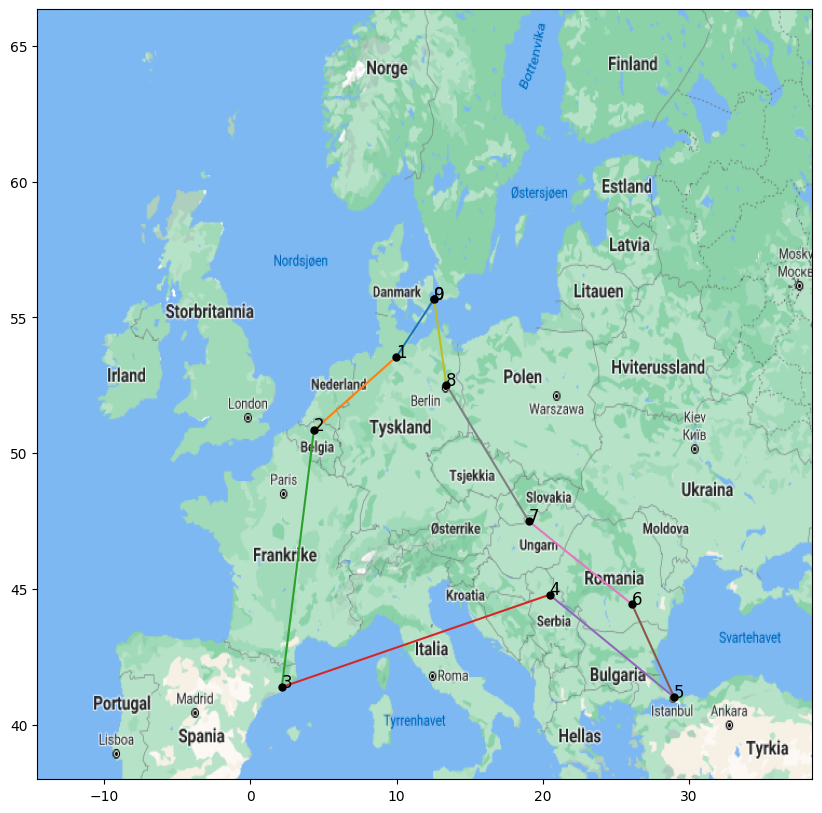
\includegraphics[width=7cm]{images/exhaustive_search_result_10_cities.png}
        \centering
        \caption{Exhaustive Search 10 cities plotted route}
    \end{figure}

    \newpage

    \subsection{Approximation for 24 cities}

    By running the code multiple times, I found out the following: 

    \begin{enumerate}
        \item 6 cities $\to$ 0:00:00.001707 $\to$ $P = 6! = 720$ routes to be checked 
        \item 8 cities $\to$ 0:00:00.123331 $\to$ $P = 8! = 40320$ routes to be checked 
        \item 9 cities $\to$ 0:00:01.006485 $\to$ $P = 9! = 362880$ routes to be checked 
        \item 10 cites $\to$ 0:00:10.756498 $\to$ $P = 10! = 3628800$ routes to be checked 
    \end{enumerate}

    I also tried with 12 cities, but it took more then 3 minutes. Clearly the growth is exponential with the permutations done for each route. 

    With 24 cites, there are $24! = 6,204484017*10^{23}$ possible routes!
    To approximate how long it would have taken for all the routes, I check how long it takes to generate one permutation and check it: 

    \[
    \text{Time per permutation}_n = \frac{\text{Total time}}{n!}
    \]

    For each test, I calculate how long it took for each permutation: 

    \[
    \text{Time per permutation for 6 cities} = \frac{0.001707}{720} \approx 2.3708 \times 10^{-6} \text{ s/route}
    \]

    \[
    \text{Time per permutation for 8 cities} = \frac{0.123331}{40320} \approx 3.0588 \times 10^{-6} \text{ s/route}
    \]

    \[
    \text{Time per permutation for 9 cities} = \frac{1.006485}{362880} \approx 2.7736 \times 10^{-6} \text{ s/route}
    \]

    \[
    \text{Time per permutation for 10 cities} = \frac{10.756498}{3628800} \approx 2.9642 \times 10^{-6} \text{ s/route}
    \]

    With this, I assume that each permutation will take the average amount of time to generate a permutation: \[2.7918\times10^{-6} \text{ s/route} \]
    Note that this might not always be correct, but I think this is a good way to approximate how long it would have taken for 24 cities. 

    Now, using this average, all me need to do is multiply the amount of permutations with the average time for each permutation to be generated: 

    \[
    \begin{aligned}
        \text{Total Time} &= 6.204484017 \times 10^{23} \times 2.7918\times10^{-6} \text{ s/route} \\
                          &= 1.73217 \times 10^{18} \text{ s}
    \end{aligned}
    \]

    To make the approximation more readable, I used a python library. 
    It has a function to make seconds into a more readable format. Link to docs: 
    \url{https://humanfriendly.readthedocs.io/en/latest/api.html#humanfriendly.format_timespan} \newline

    Using the function to get the total time in a readable format, shows how long time 24 cities with exhaustive search would have taken: \textbf{55077648046 years, 20 weeks and 4 days}.

    \section{Hill Climbing}

    Hill Climbing is an algorithm that combines randomness and greedy search into a single algorithm.
    This is how my implementation works:
    \begin{itemize}
        \item Create a random initial route (valid route only)
        \item Store the best route in a variable. For each of the 20 runs: 
        \begin{itemize}
            \item Create a neighbor solution by swapping two random cities. The cities swapped are not the start city. 
            \item Evaluate this neighbor solution, and set it as the best route, if the distance is smaller
        \end{itemize}
    \end{itemize}


    There is a lot of different ways to create a random neighbor solution. By experimenting, it turns out that swapping to cities on the current best solution is a good idea. 
    It converges towards a better solution. It is still important to run it 20 times, because it has a random element to it. 

    \subsection{Performance compared to Exhaustive Search (10 cities)}

    Hill climbing compared to Exhaustive Search, does not look at every solution. This means both that it is less likely to find the best solution.
    With 10 cities are the total search space much smaller. It took $\sim1.6$ seconds to find the best distance 7486.309 km. Even though we found the same solution as Exhaustive Search, there is a difference in time spent.
    Exhaustive Search used  $\sim13.48$ seconds (compared to the   $\sim1.6$ seconds).

    The only flaw with the Hill Climbing algorithm, is that we need to run it multiple times to get a deterministic result. This is because the Hill Climbing algorithm has a random element to it. 
    20 runs seems to be enough to get the same best route as exhaustive search 


    \subsection{Result for 10 and 24 cities (20 runs each)}

    The following is a table showing the result for both runs:

    \begin{table}[ht]
        \centering
        \resizebox{\textwidth}{!}{
            \begin{tabular}{|c|c|c|c|c|c|}
                \hline
                \textbf{Number of Cities} & \textbf{Best Distance} & \textbf{Average Distance} & \textbf{Worst Distance} & \textbf{Std. Deviation} & \textbf{Time Taken (s)} \\ \hline
                \textbf{10 Cities}        & 7486.31     & 7825.79     & 8421.35     & 405.37            & $\sim1.6$             \\ \hline
                \textbf{24 Cities}        & 13347.75    & 15083.53    & 17177.85    & 1079.74           & $\sim2.2$             \\ \hline
            \end{tabular}
        }
        \caption{Hill Climbing results for 10 and 24 cities (20 runs each)}
    \end{table}
    

    Images below are plotted routes of the best routes from a run: 

    \begin{figure}[ht]
        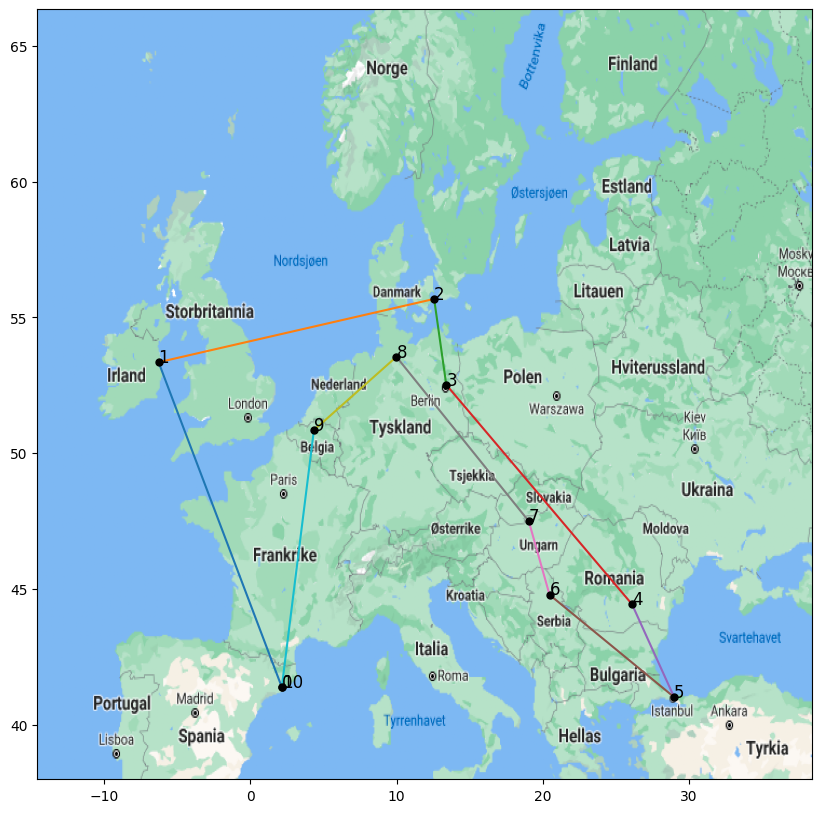
\includegraphics[width=7cm]{images/hill_climb_10_cities.png}
        \centering
        \caption{Hill climb 10 cities plotted route}
    \end{figure}


    \begin{figure}[ht]
        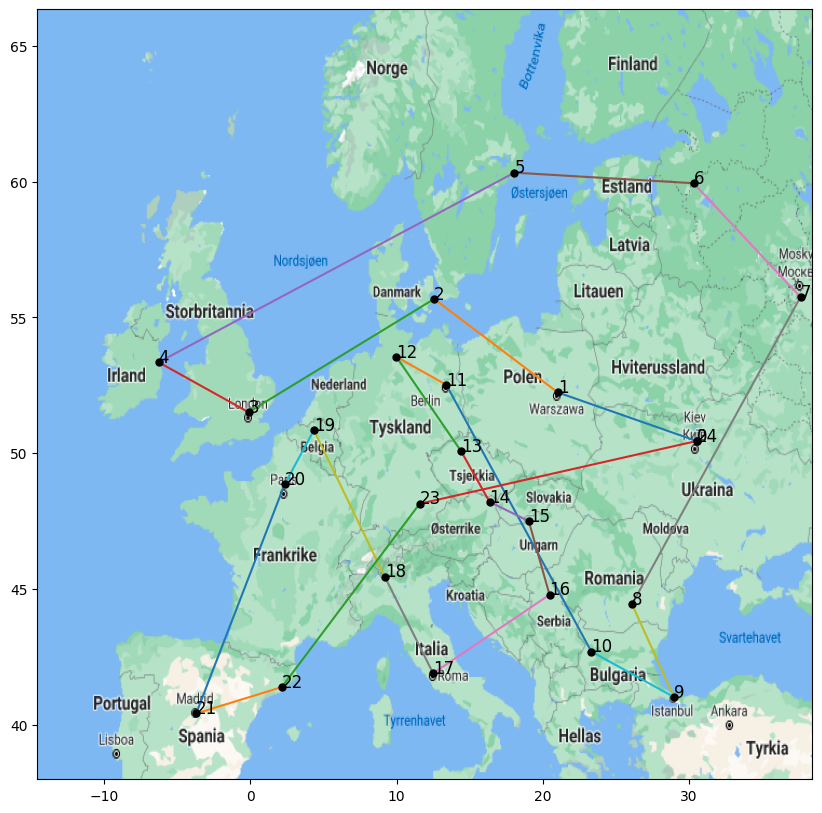
\includegraphics[width=7cm]{images/hill_climb_24_cities.png}
        \centering
        \caption{Hill climb 24 cities plotted route}
    \end{figure}




    \section{Genetic algorithm}

    Genetic algorithm is very inspired by evolutions, and is very useful for both search problems where a combination of exploration and exploitation is useful.
    There is many different tricks and variations when it comes to the algorithm. Based on the problem, the developer can implement domain specific elements to the algorithm. For example, picking a specific mutation method based on the understanding of the problem. \\
    
    Genetic algorithm is flexible, but still follows the general scheme. For each part of the scheme, I will explain what I did, some experimenting I did and reason on why I choose the given method for the traveling salesman problem.

    \begin{figure}[ht]
        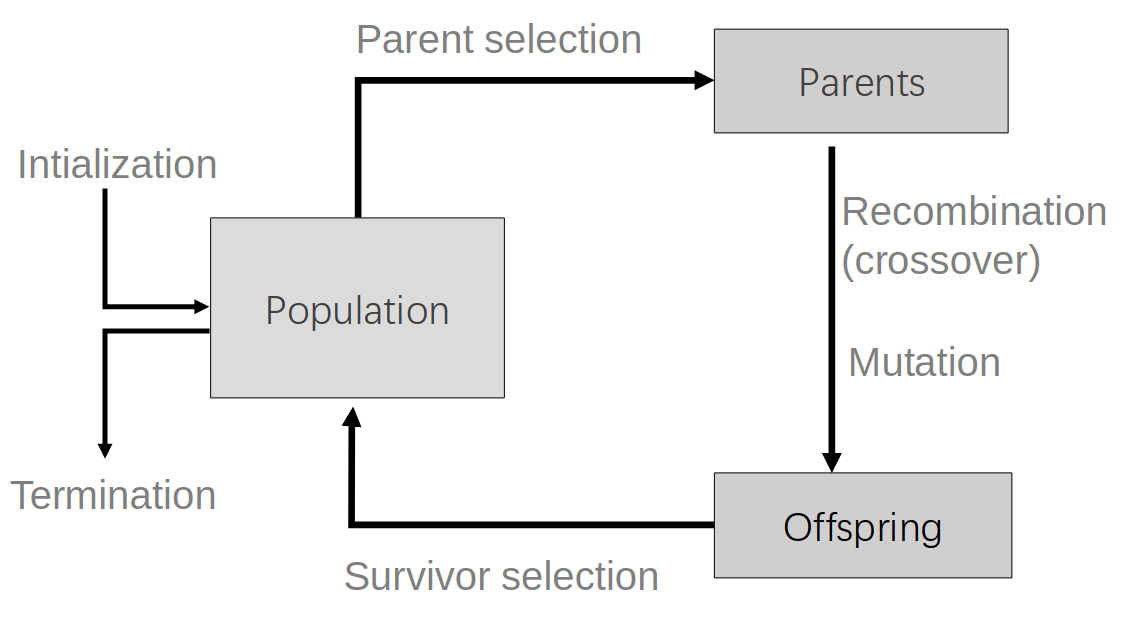
\includegraphics[width=7cm]{images/ga_scheme.png}
        \centering
        \caption{GA scheme for reference}
    \end{figure}


    \subsection{Create initial population}

    \subsection{Parent Selection}

    \subsection{Crossover}

    \subsection{Mutation}

    \subsection{Survivor Selection}

    \subsection{Termination}

    \subsection{Results: 10 cities}

    \subsection{Results: 24 cities}

    \subsection{GA compared to Exhaustive Search}




\end{document}